\chapter{Ist-Analyse ( 5 \%)}
\label{chap:ist-analyse}

Dieses Kapitel dient der Beschreibung existierender System.
Es soll ihre Eigenschaften und Probleme aufzeigen.
Diese werden zuerst Theoretisch betrachtet und
dann an Systemen in der Praxis demonstriert.

% dieses kap dient .. und damit soll .. aufbau

\section{Eigenschaften der existierenden Systeme}

\subsection{Struktur}
Wie in der folgenden Grafik leicht zu erkennen,

\begin{figure}[ht]
  \centering
  \label{fig:ist-aufbau-tradition}
  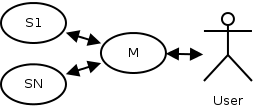
\includegraphics[height=1in]{imageinput/ist-aufbau-tradition.png}
  \caption{Logischer Aufbau eines CI System}
\end{figure}

\subsection{Datensammlung}

\begin{verbatim}
- datensammlung
  - logs
    - in time
    - STDOUT,
  - files
    - junitxml
\end{verbatim}

\section{Probleme existierender Systeme}


\subsection{Datenzugriff}

\begin{verbatim}
- eigene datenformate
- dumb stores
\end{verbatim}

\subsection{Erweiterbarkeit}
\begin{verbatim}

\end{verbatim}


\subsection{Komponentenabh\"angigkeit}
\begin{verbatim}
  - strikt master/slave
  - client/server prob
  - zentrales management
  - alles wird im master gemanagt
  - dumme arbeiter, keinerlei autonomie

  - ausfall von master bedingt ausfall von slave


\end{verbatim}

\section{Praxisbeisiele}

\subsection{Auswahl}

\begin{verbatim}

- opensource/oeffentlich
\end{verbatim}

\subsection{Jenkins}

\begin{verbatim}
pro:
- build matrix
- ui

cons:
- datenzugriff
- erweiterungen
- dateninteraktion?

\end{verbatim}

%XXX referenzen
Jenkins und Hudson stellen ein Benutzerfreundliches,
jedoch limitiertes System zum einfachen Anlegen von Build-Jobs.

Parametrisierung ist nicht möglich.

\subsection{Buildbot}


\begin{verbatim}
pro:
- flexible builds
- rudimentaerer datenzugriff
- parameter (z.b. branch)
cons:
- datenmodell
- ui


- beispiel pypy uebersicht

\end{verbatim}


%XXX referenzen
BuildBot positioniert sich als eine Art Meta-Build-Server.
es biete keine normale Oberfläche, sondern wird mittels
Komposition von Metadaten und Komponenten konfiguriert.

Die Konfiguration des Servers stellt dabei ein Python script,
welches die Operationen ausführt, welche zur Zusammenstellung des gewünschten Servers notwendig sind.

Es ist möglich Builds Jobs mit minimale Parameter in Form von Strings zu Übergeben.

\subsection{TravisCI}

\begin{verbatim}
pro:
- ui
  - screenshoot
- matix builds
- branch builds -> via pull req

cons
- mangel an datenzugriff
- hosted
- nicht portabel
\end{verbatim}



\section{Zusammenfassung}

% Dieses Kap. hat getz ..

% wie haben gesehen das ..

% im folgenden verlauf der arbeit \ldots
% 2-3 saetze
